\section{Urbana-Champaign and UIUC}

\subsection{About Urbana-Champaign}
Champaign-Urbana (CU) is a close-knit community filled with music, culture, and food. While Campustown, the neighborhood immediately surrounding campus,  is an important part of the atmosphere, there is plenty to do off campus. Relax in one of the outdoor restaurants downtown or walking through the various gardens and parks around town. The culture in Champaign is very rich as a result of many annual festivals such as the CU Pride Parade, the Ellnora guitar festival, and the Pygmalion festival. The Krannert Center for the Performing Arts is also a world-renowned theater that has hosted groups from all genres like the New York Philharmonic, the Russian National Ballet, and Sonny Rollins.

\subsubsection{Accessibility}
Myriad festivals and sporting events on campus draw many people to Champaign-Urbana at varying times of the year, which means hotels are not hard to find. A large number of these hotels are located around downtown Champaign and the Eastern side of campus, making transportation easy. There is also a small airport, Willard Airport, just 20 minutes from campus that regularly has flights to and from the Chicago O’Hare and Dallas Ft Worth airports. Finally, there are several reliable bus services that make frequent trips from Champaign-Urbana to O’Hare and the Chicagoland area.

\subsubsection{Weather}
With an average high temperature of 65$^{\circ}$ and an average low temperature of 40$^{\circ}$, April in Champaign is a gorgeous month of dwindling winter weather as summer begins to round the corner. Holding a conference during this time would be the perfect way to showcase our beautiful city.

\subsection{About the University of Illinois}
Founded in 1867, the University of Illinois at Urbana-Champaign (UIUC) has cultivated a long history of significant scientific discoveries and contributions. The theory of superconductivity, the invention of the transistor, the discovery of archaea, the fourth domain of life, and the first web browser are just some of the many breakthroughs from UIUC. Established in 1876, the famous Morrow Plots became the first research crop field at a university and is still used today. Attendees will also be familiar with Blue Waters, one of the world’s fastest supercomputers. 
The UIUC Grainger College of Engineering has had sixteen Nobel Laureates in physics. Including John Bardeen, the only scientist to ever win the award twice. It also offers 15 different majors to more than 9,100 undergraduate and 3,400 graduate students. Of its twelve ranked majors, nine are ranked among the top 10 in the nation, and six of which remain ranked among the top 5 in their degree. Overall, the College of Engineering in Urbana-Champaign ranks sixth among the nation’s best undergraduate engineering programs. With more than 250 degrees for undergraduates and graduates and a multitude of first-class research facilities and resource, UIUC gives its 45,000 students the ability to succeed.\\
Today, the University of Illinois at Urbana-Champaign attracts visitors from throughout the state by offering a variety of valuable public attractions. UIUC maintains four public museums: the Spurlock Museum, containing 54,000 cultural artifacts from around the world; the Illinois Natural History Survey, has more than 9.5 million biologic specimens in its collection; the Sousa Archives and Center for American Music, provides shows and education to students and the public; and the Krannert Art Museum, offers fine arts and education. More than 470,000 square feet of recreational space is occupied by other facilities including an ice arena, climbing wall, swimming pools, parks, sports fields, parks, and outdoor adventure venues. 

\subsection{UIUC ANS Student Chapter (ANS-UIUC)}
The ANS-UIUC maintains and develops a cohesive community of students in nuclear engineering. It also engages in education and outreach programs to teach members of the surrounding community about nuclear science. Membership is currently around 70-80 students and has been steadily growing. The chapter works to host events catering to nuclear, plasma, and radiological concentrations. It also makes professional development a large part of member involvement. ANS-UIUC has historically been one of the best represented institutions at the annual student conference and is a tradition this chapter is eager to uphold. 

% Group picture from the 2019 kick off barbeque.
\begin{figure}[H]
	\centering
	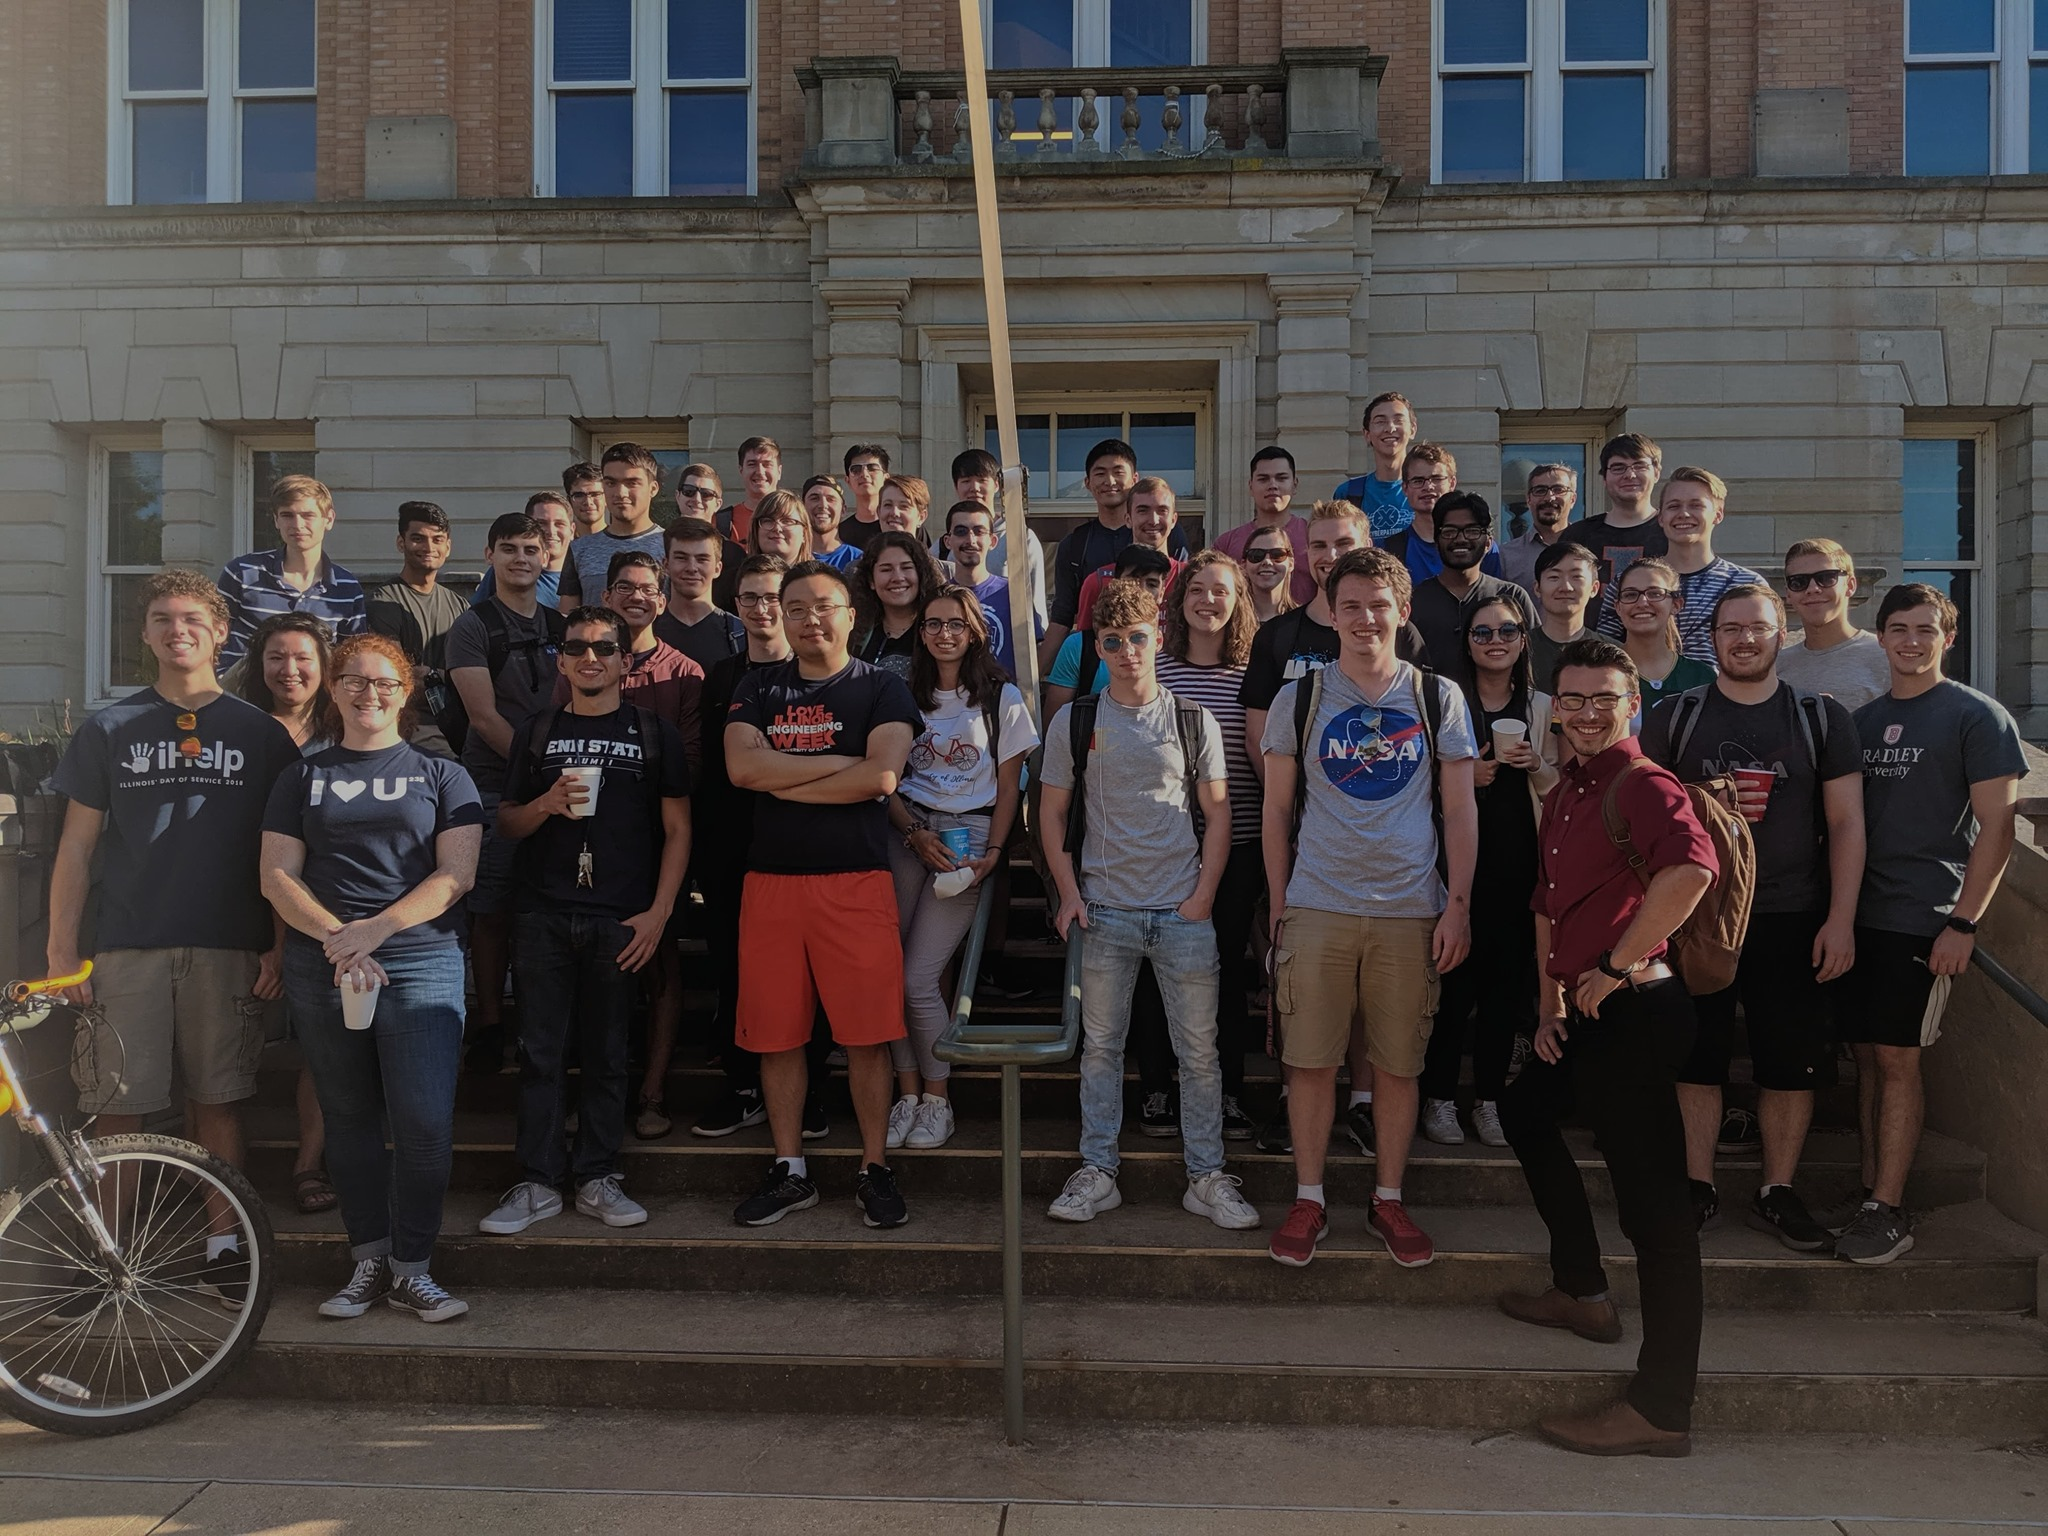
\includegraphics[width=9cm]{ans_uiuc_group.jpg}
\end{figure}

% Picture of attendees to the 2019 ANS Student Conference
\begin{figure}[H]
	\centering
	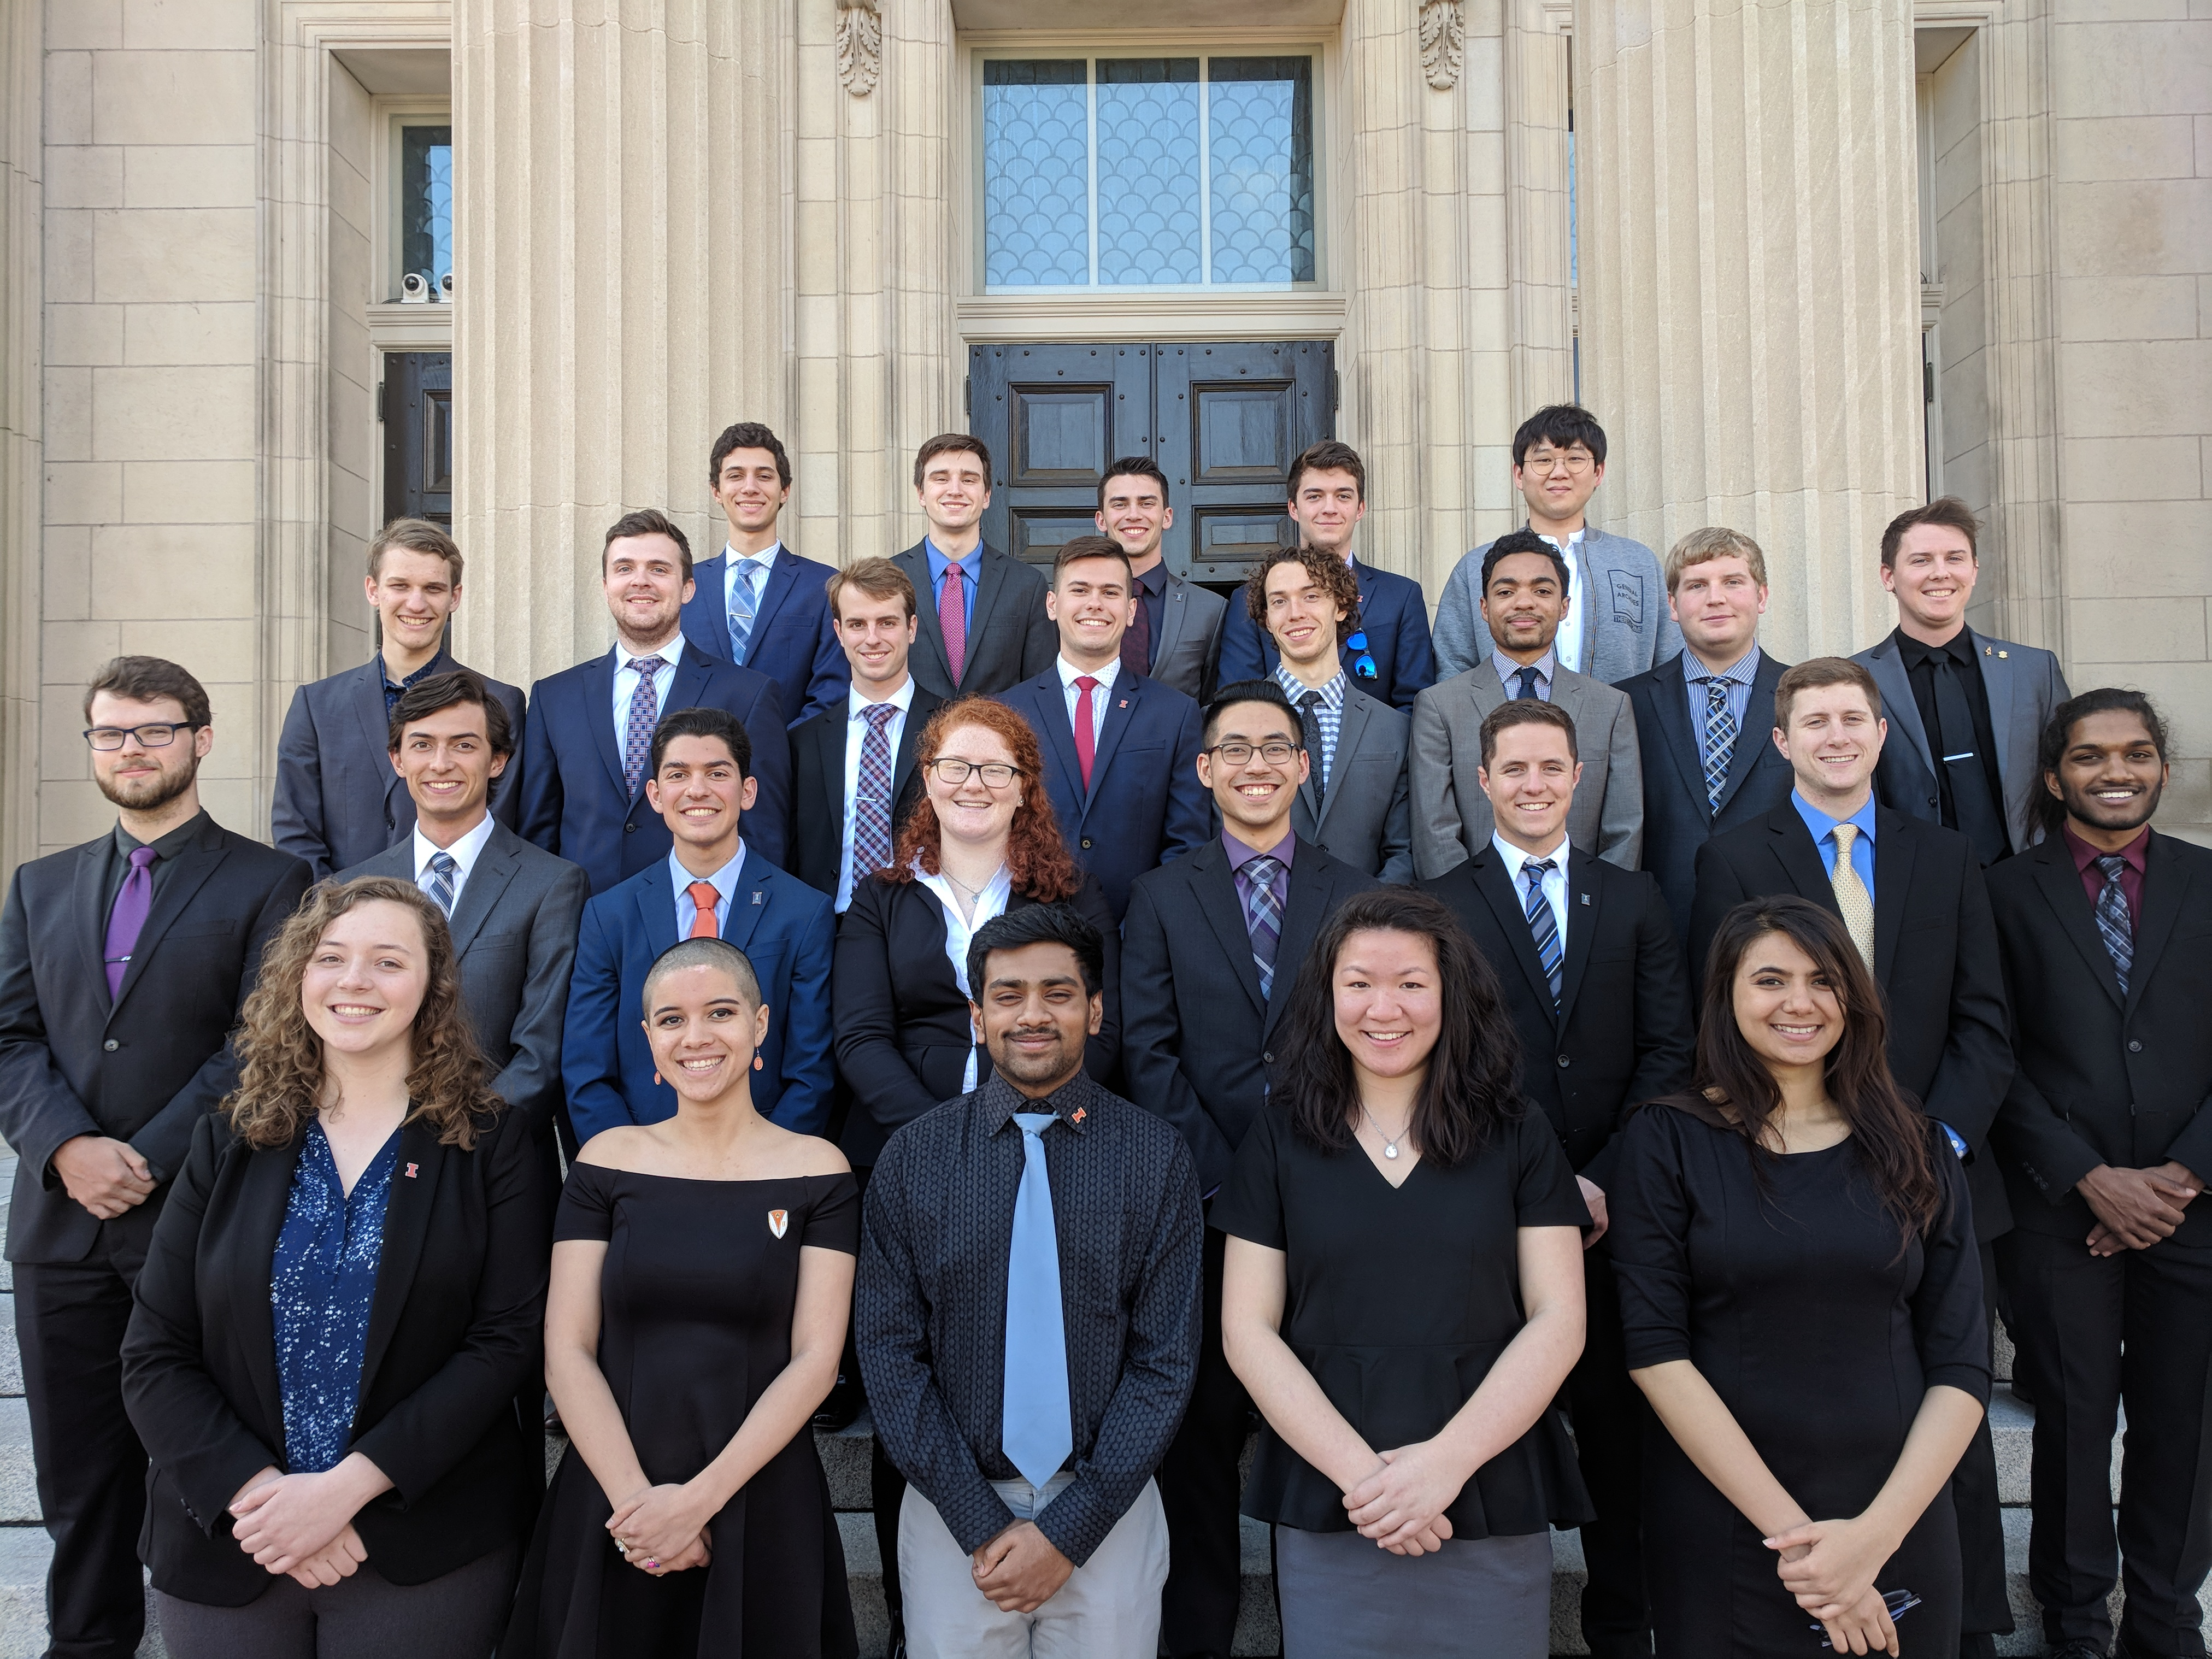
\includegraphics[width=9cm]{ans_conf_19.jpg}
\end{figure}
